
In this section, the results of the regression cases (burnup, enrichment, and
time since irradiation) are presented. For each prediction parameter, the plot
format described in Figure \ref{fig:detdemo} is used to show both the
\gls{MAPE} for each of the three energy window lists.  However, while seeing
the performance decrease with all three algorithms on the same plot is helpful
for getting a bigger picture of the results, a more detailed visual is also
helpful. 

Introduced in Section \ref{sec:sfcoreg}, box plots provide increased
statistical detail and a direct comparison of mean and median error for each
data point, which each taken alone can paint a drastically different picture of
the results.  There is one set of boxes for each algorithm for a given energy
window list-based set of detector training sets.  Because these are box plots,
they are not oriented to the "higher is better" standard of the \textit{y}-axis
of the original prediction performance plots.  There are the same red
baselines, but they are now at a positive value since the \textit{y}-axis is no
longer negative.  Lastly, the full knowledge cases (the 29 nuclide masses, and
the 32, 12, and 7 nuclide activities sets) are not able to be represented on
the same scale as the detector training set results, so they are excluded from
the box plot figures. 

Lastly, in order to see the spread of the data and compare the mean and median
errors, the outliers were supressed from the box plots. There are many outliers
in these results, and the values can be quite large. Each set of box plots is
therefore repeated with a set of box plots with the outliers included.

\subsubsection{Burnup Regression}

The baseline performance in Figure \ref{fig:burn} is at -4\% \gls{MAPE} for
burnup, chosen by the lowest performance of the three algorithms at the
reference point of 20\% training set error for the 29 nuclide mass training set
in in Figure \ref{fig:randerrB}. In Figures \ref{fig:burnbox} and
\ref{fig:burnboxfly}, the red baseline is at $1000\:MWd/MTU$, from the
reference point in Figure \ref{fig:randmaeA}.  In these two sets of plots, the
baseline is at a positive value because the box plots do not have a negative
\textit{y}-axis. 

Figure \ref{fig:burn} shows encouraging results about the burnup prediction,
for all three algorithms and all three energy windows lists used to process the
gamma spectra. There is overall a gradual decrease from perfect knowledge
starting at close to 0\% error to the lowest energy resolution detector at
about -1.5\%.  There are two anomalous cases, as with the reactor type results
in Figure \ref{fig:rxtr}: the predictions using \textit{k}-nearest neighbors
for the two \gls{HPGe} detectors processed with the auto energy windows list.
The reason for this behavior is discussed at the end of Section
\ref{sec:exp2_rxtr}. 

\begin{figure}[!htb]
  \centering
  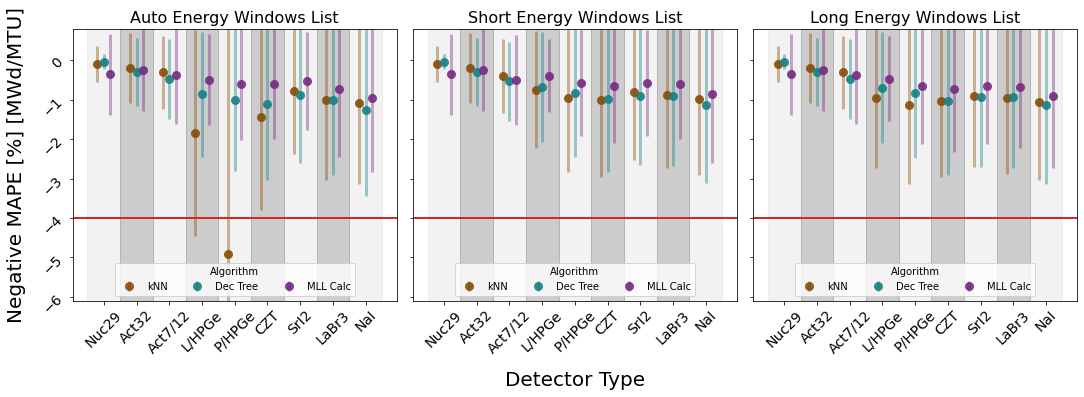
\includegraphics[width=\textwidth]{./chapters/exp2/detector_preds_wrt_enlist_MAPE_burn.png}
  \caption{Prediction performance of burnup measured by \gls{MAPE} with 
           respect to decreasing detector energy resolution for three types 
           of processed gamma spectra.}
  \label{fig:burn}
\end{figure}

\begin{figure}[!hp]
  \centering
  \begin{subfigure}[b]{\textwidth}
    \centering
    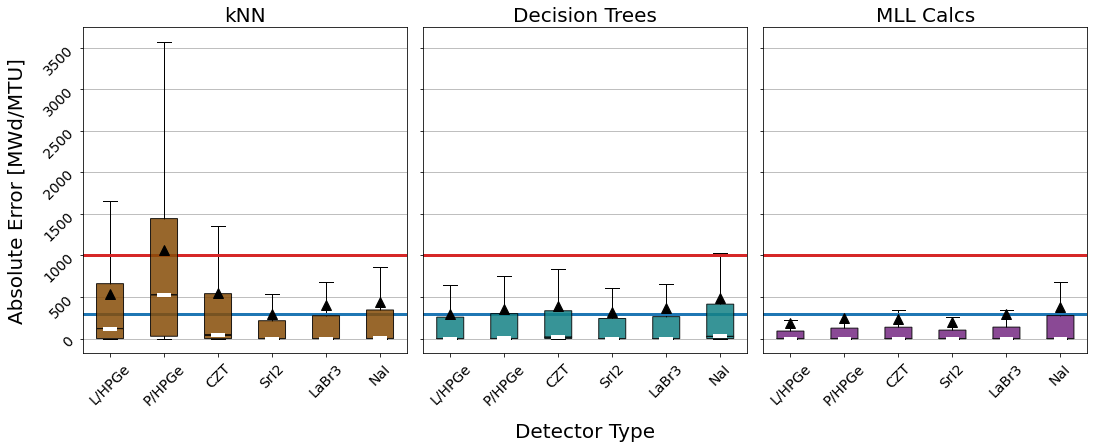
\includegraphics[width=0.92\textwidth]{./chapters/exp2/abserror_boxplots_auto_burn.png}
    \caption{Burnup prediction error box plots for auto energy windows list.}
    \label{fig:burnboxA}
  \end{subfigure}
  \vskip\baselineskip
  \begin{subfigure}[b]{\textwidth}
    \centering
    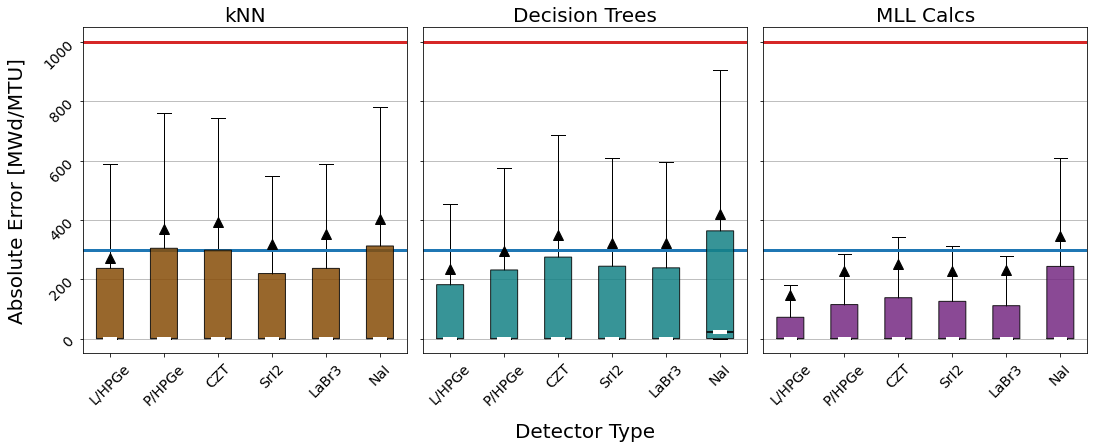
\includegraphics[width=0.92\textwidth]{./chapters/exp2/abserror_boxplots_short_burn.png}
    \caption{Burnup prediction error box plots for short energy windows list.}
    \label{fig:burnboxB}
  \end{subfigure}
  \vskip\baselineskip
  \begin{subfigure}[b]{\textwidth}
    \centering
    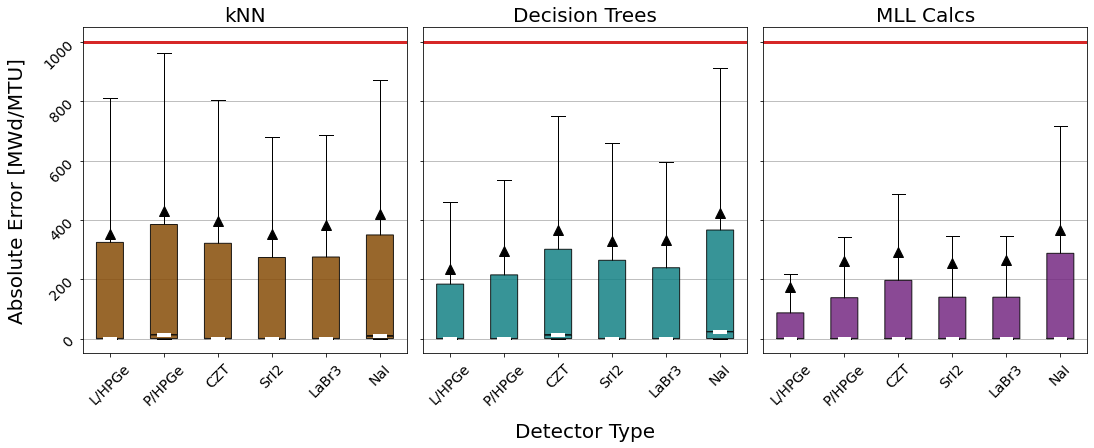
\includegraphics[width=0.92\textwidth]{./chapters/exp2/abserror_boxplots_long_burn.png}
    \caption{Burnup prediction error box plots for long energy windows list.}
    \label{fig:burnboxC}
  \end{subfigure}
  \caption{Prediction performance of burnup for six detectors as shown by box 
           plots.}
  \label{fig:burnbox}
\end{figure}

\begin{figure}[!hp]
  \centering
  \begin{subfigure}[b]{\textwidth}
    \centering
    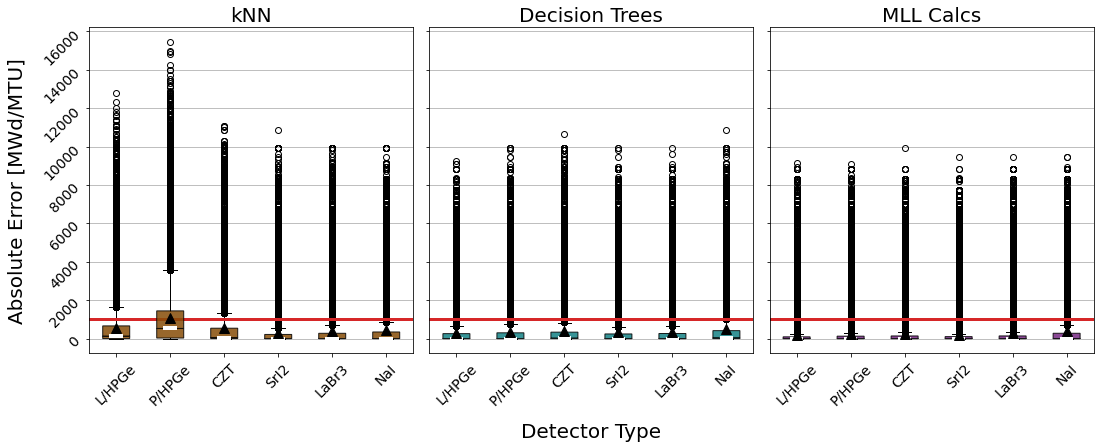
\includegraphics[width=0.92\textwidth]{./chapters/exp2/abserror_boxplots_outliers_auto_burn.png}
    \caption{Burnup prediction error box plots for auto energy windows list.}
    \label{fig:burnboxflyA}
  \end{subfigure}
  \vskip\baselineskip
  \begin{subfigure}[b]{\textwidth}
    \centering
    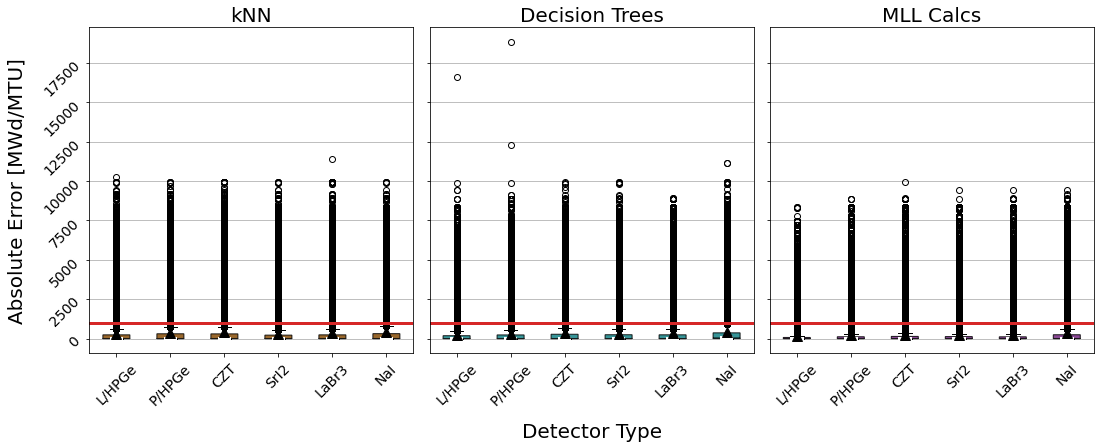
\includegraphics[width=0.92\textwidth]{./chapters/exp2/abserror_boxplots_outliers_short_burn.png}
    \caption{Burnup prediction error box plots for short energy windows list.}
    \label{fig:burnboxflyB}
  \end{subfigure}
  \vskip\baselineskip
  \begin{subfigure}[b]{\textwidth}
    \centering
    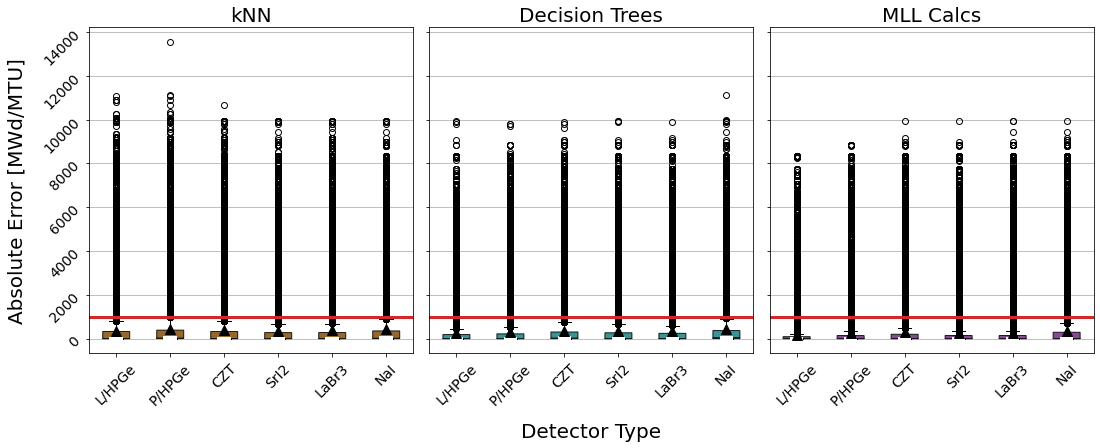
\includegraphics[width=0.92\textwidth]{./chapters/exp2/abserror_boxplots_outliers_long_burn.png}
    \caption{Burnup prediction error box plots for long energy windows list.}
    \label{fig:burnboxflyC}
  \end{subfigure}
  \caption{Prediction performance of burnup for six detectors as shown by box 
           plots.}
  \label{fig:burnboxfly}
\end{figure}

Next, the \textit{y}-axis orientation flips to positive absolute error, so that
higher values are worse and the goal is to have the mean and median errors be
below the red line.  Most of the burnup errors in Figures \ref{fig:burnboxA},
\ref{fig:burnboxB}, and \ref{fig:burnboxC} are below the red line, except for
the mean error from the portable \gls{HPGe}


\subsubsection{U235 Enrichment Regression}

The baseline performance for the enrichment predictions in Figure
\ref{fig:enri} is at -6\% \gls{MAPE}, chosen by the lowest performance of the
three algorithms at the reference point of 20\% training set error for the 29
nuclide mass training set in in Figure \ref{fig:randerrC}. In Figures
\ref{fig:enribox} and \ref{fig:enriboxfly}, the red baseline is at $0.17\:[\%
U235]$, from the reference point in Figure \ref{fig:randmaeB}.  In these two
sets of plots, the baseline is at a positive value because the box plots do not
have a negative \textit{y}-axis. 

\begin{figure}[!htb]
  \centering
  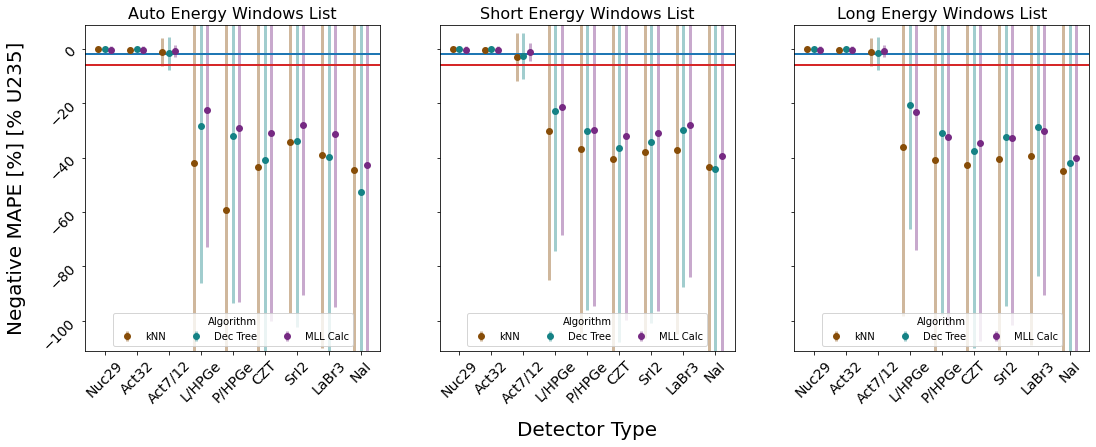
\includegraphics[width=\textwidth]{./chapters/exp2/detector_preds_wrt_enlist_MAPE_enri.png}
  \caption{Prediction performance of \gls{U235} enrichment measured by 
           \gls{MAPE} with respect to decreasing detector energy resolution 
           for three types of processed gamma spectra.}
  \label{fig:enri}
\end{figure}

Taken as a whole, the data points in Figure \ref{fig:enri} have a distinct
shape, similar to the behavior in Figue \ref{fig:rxtr}.  The three full
knowledge cases have near-perfect enrichment prediction and the six detectors
for all three energy windows lists are nearly flat. For both Figures
\ref{fig:enri}, the blue line is therefore not making any
meaningful discrimination. The almost even performance across detector types 
and algorithms (with exceptions) \todo{left off here}

As with the other previously discussed prediction types, there are two
anomalous cases: the prediction using \textit{k}-nearest neighbors for the two
\gls{HPGe} detectors processed with the auto energy windows list. The reason
for this behavior is discussed at the end of Section \ref{sec:exp2_rxtr}. 

\begin{figure}[!hp]
  \centering
  \begin{subfigure}[b]{\textwidth}
    \centering
    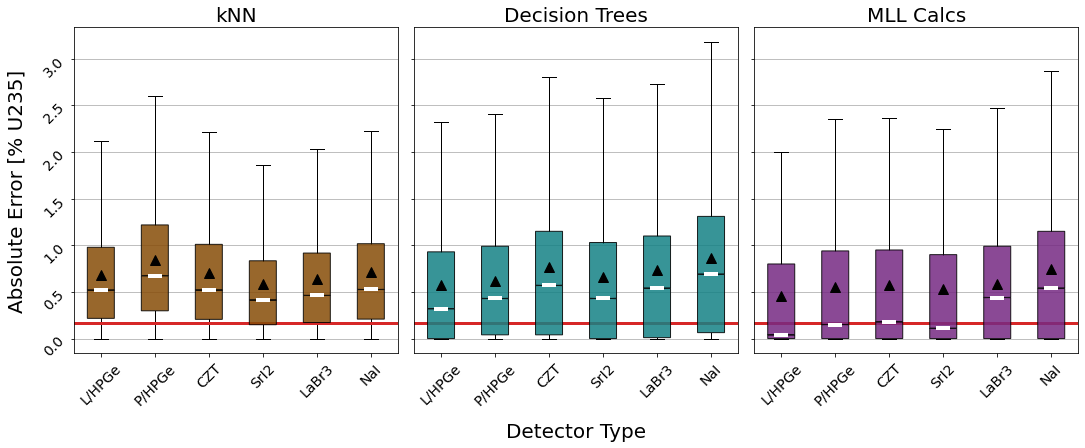
\includegraphics[width=0.92\textwidth]{./chapters/exp2/abserror_boxplots_auto_enri.png}
    \caption{\gls{U235} enrichment prediction error box plots for auto energy windows list.}
    \label{fig:enriboxA}
  \end{subfigure}
  \vskip\baselineskip
  \begin{subfigure}[b]{\textwidth}
    \centering
    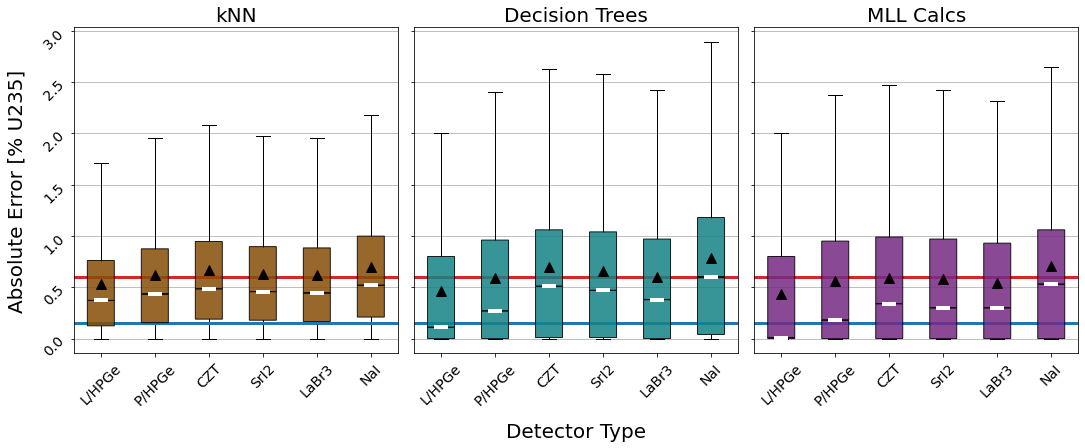
\includegraphics[width=0.92\textwidth]{./chapters/exp2/abserror_boxplots_short_enri.png}
    \caption{\gls{U235} enrichment prediction error box plots for short energy windows list.}
    \label{fig:enriboxB}
  \end{subfigure}
  \vskip\baselineskip
  \begin{subfigure}[b]{\textwidth}
    \centering
    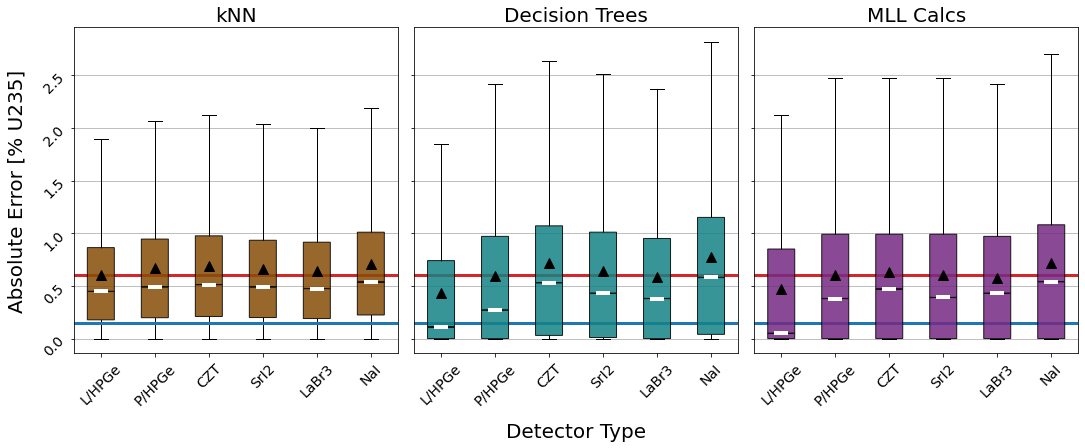
\includegraphics[width=0.92\textwidth]{./chapters/exp2/abserror_boxplots_long_enri.png}
    \caption{\gls{U235} enrichment prediction error box plots for long energy windows list.}
    \label{fig:enriboxC}
  \end{subfigure}
  \caption{Prediction performance of \gls{U235} enrichment for six detectors as 
           shown by box plots.}
  \label{fig:enribox}
\end{figure}

\begin{figure}[!hp]
  \centering
  \begin{subfigure}[b]{\textwidth}
    \centering
    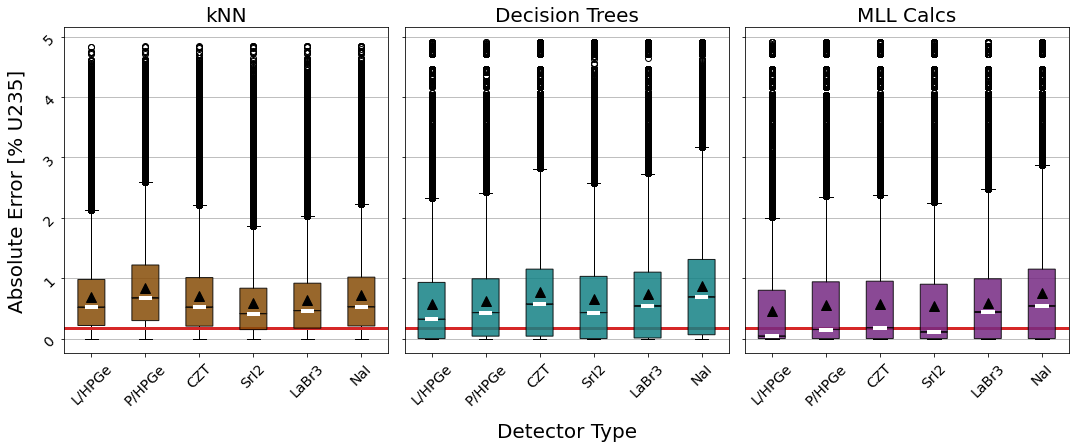
\includegraphics[width=0.92\textwidth]{./chapters/exp2/abserror_boxplots_outliers_auto_enri.png}
    \caption{\gls{U235} enrichment prediction error box plots for auto energy windows list.}
    \label{fig:enriboxflyA}
  \end{subfigure}
  \vskip\baselineskip
  \begin{subfigure}[b]{\textwidth}
    \centering
    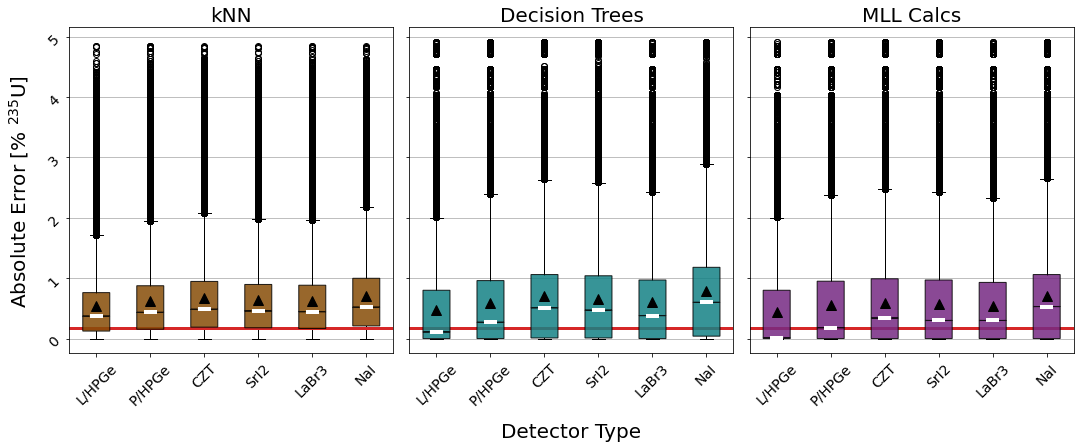
\includegraphics[width=0.92\textwidth]{./chapters/exp2/abserror_boxplots_outliers_short_enri.png}
    \caption{\gls{U235} enrichment prediction error box plots for short energy windows list.}
    \label{fig:enriboxflyB}
  \end{subfigure}
  \vskip\baselineskip
  \begin{subfigure}[b]{\textwidth}
    \centering
    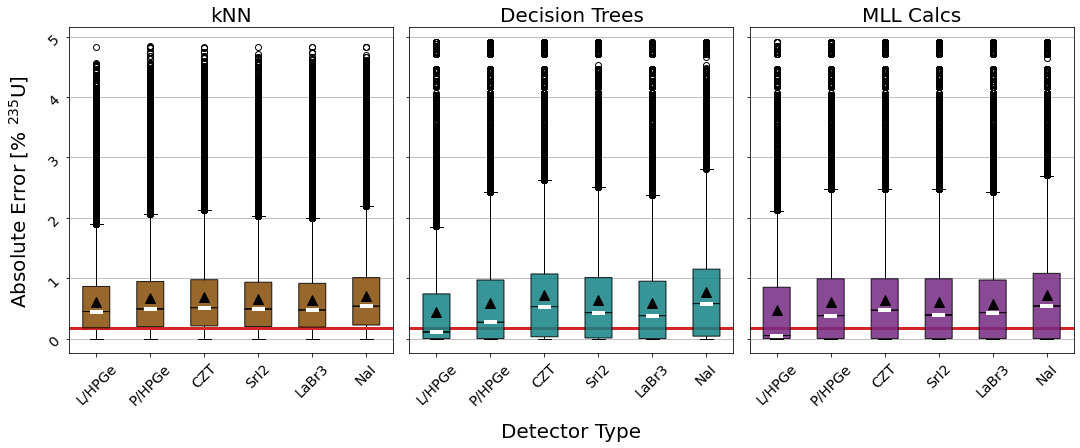
\includegraphics[width=0.92\textwidth]{./chapters/exp2/abserror_boxplots_outliers_long_enri.png}
    \caption{\gls{U235} enrichment prediction error box plots for long energy windows list.}
    \label{fig:enriboxflyC}
  \end{subfigure}
  \caption{Prediction performance of \gls{U235} enrichment for six detectors as 
           shown by box plots.}
  \label{fig:enriboxfly}
\end{figure}

\subsubsection{Time Since Irradiation Regression}

The original baseline performance for the time since irradition predictions in
Figure \ref{fig:cool} were at -30\% \gls{MAPE}, chosen by the lowest
performance of the three algorithms at the reference point of 20\% training set
error for the 29 nuclide mass training set in in Figure \ref{fig:randerrD}.
However, the \textit{k}-nearest neighbors algorithm in that plot had
exceptionally poor performance compared to the other two algorithms, so all of
the results from the detector-based training sets (including those predicted
using \textit{k}-nearest neighbors, oddly enough) far outperform this baseline.
Therefore, a new one was chosen based on the decision trees performance at the
reference point in Figure \ref{fig:randerrD}, at a \gls{MAPE} of -6\%.
Similarly, in Figures \ref{fig:coolbox} and \ref{fig:coolboxfly}, the original
baseline is at $550\:[days]$ and the updated red baseline is at $120\:[days]$,
from the \textit{k}-nearest neighbors and decision trees performances,
respectively, at the reference point in Figure \ref{fig:randmaeC}.  In these
two sets of plots, the baseline is at a positive value because the box plots do
not have a negative \textit{y}-axis. 

\begin{figure}[!htb]
  \centering
  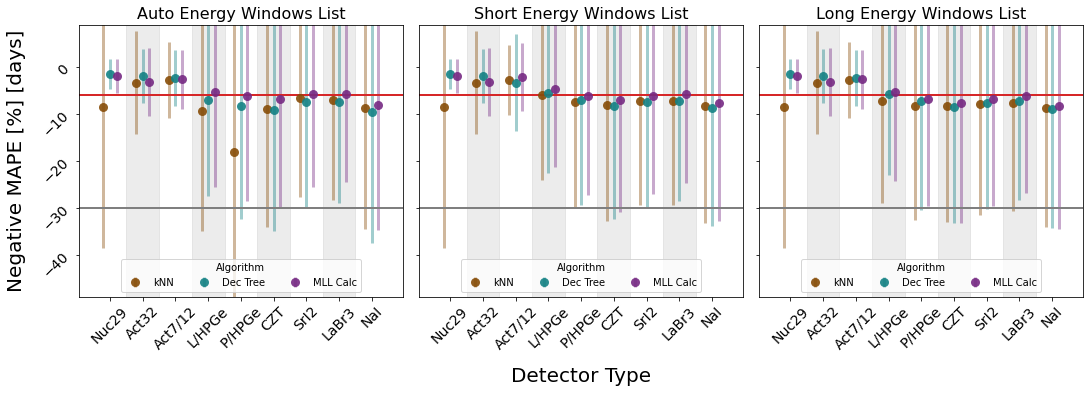
\includegraphics[width=\textwidth]{./chapters/exp2/detector_preds_wrt_enlist_MAPE_cool.png}
  \caption{Prediction performance of time since irradiation measured by 
           \gls{MAPE} with respect to decreasing detector energy resolution 
           for three types of processed gamma spectra.}
  \label{fig:cool}
\end{figure}

As with the other previously discussed prediction types, there are two
anomalous cases: the prediction using \textit{k}-nearest neighbors for the two
\gls{HPGe} detectors processed with the auto energy windows list. The reason
for this behavior is discussed at the end of Section \ref{sec:exp2_rxtr}. 

\begin{figure}[!hp]
  \centering
  \begin{subfigure}[b]{\textwidth}
    \centering
    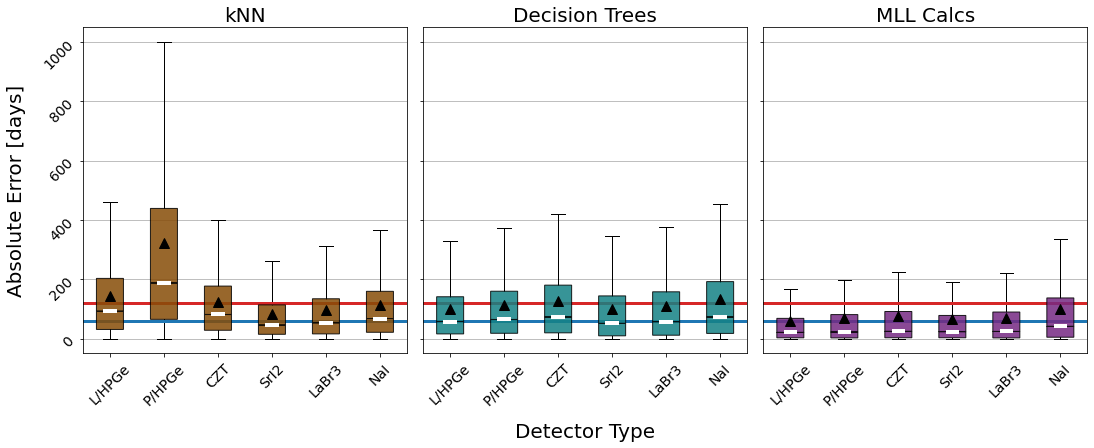
\includegraphics[width=0.92\textwidth]{./chapters/exp2/abserror_boxplots_auto_cool.png}
    \caption{Time since irradiation prediction performance box plots for auto energy windows list.}
    \label{fig:coolboxA}
  \end{subfigure}
  \vskip\baselineskip
  \begin{subfigure}[b]{\textwidth}
    \centering
    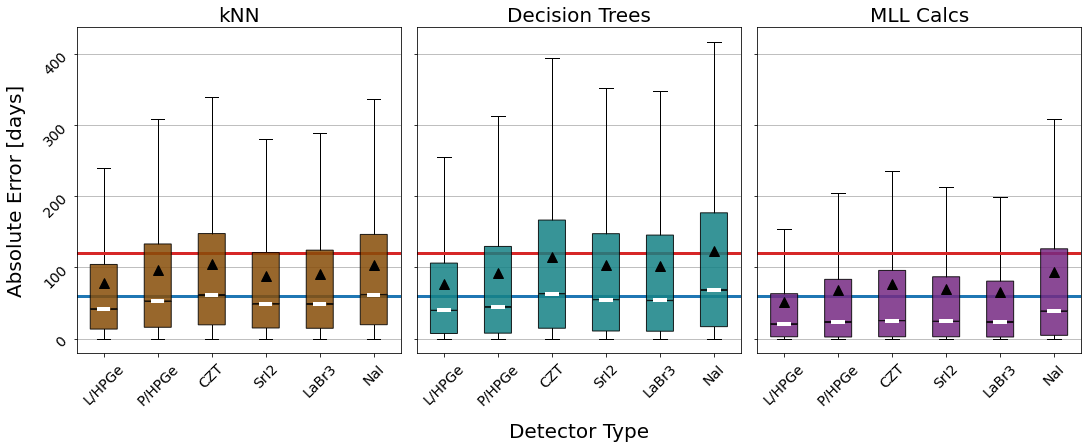
\includegraphics[width=0.92\textwidth]{./chapters/exp2/abserror_boxplots_short_cool.png}
    \caption{Time since irradiation prediction performance box plots for short energy windows list.}
    \label{fig:coolboxB}
  \end{subfigure}
  \vskip\baselineskip
  \begin{subfigure}[b]{\textwidth}
    \centering
    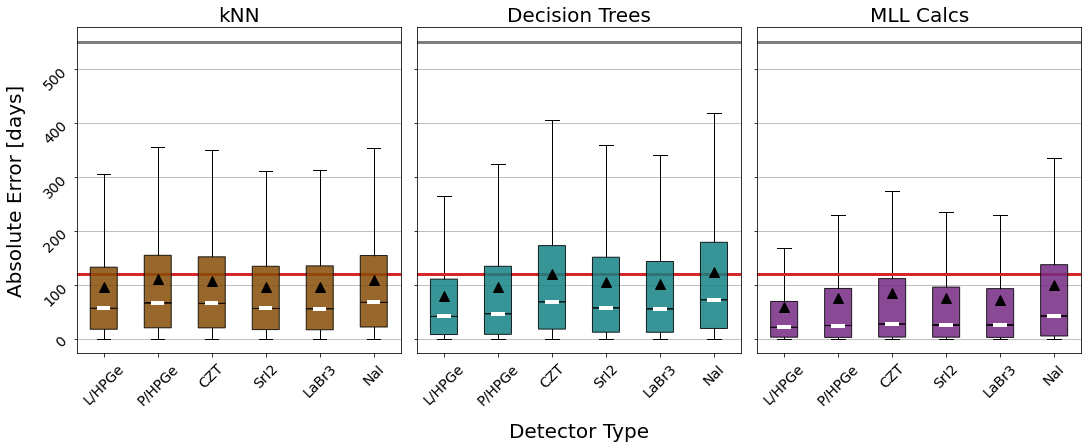
\includegraphics[width=0.92\textwidth]{./chapters/exp2/abserror_boxplots_long_cool.png}
    \caption{Time since irradiation prediction performance box plots for long energy windows list.}
    \label{fig:coolboxC}
  \end{subfigure}
  \caption{Prediction performance of time since irradiation for six detectors as 
           shown by box plots.}
  \label{fig:coolbox}
\end{figure}

\begin{figure}[!hp]
  \centering
  \begin{subfigure}[b]{\textwidth}
    \centering
    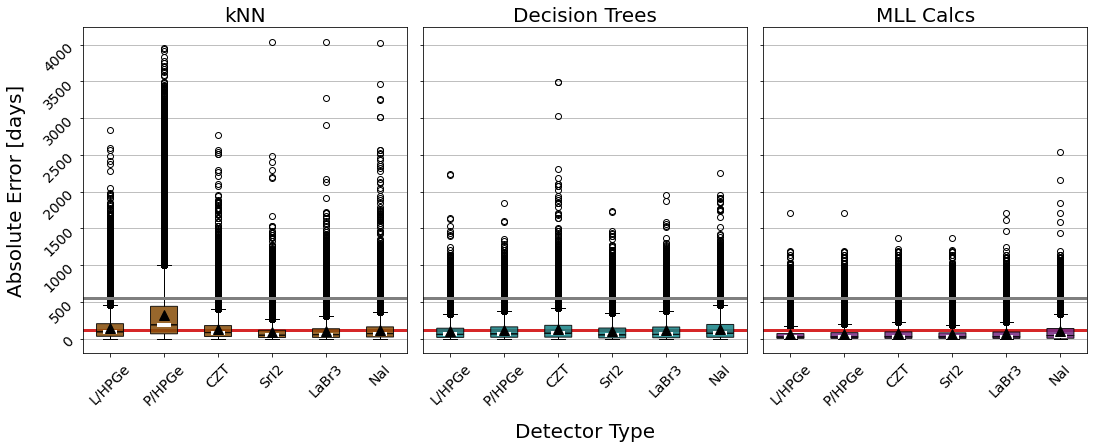
\includegraphics[width=0.92\textwidth]{./chapters/exp2/abserror_boxplots_outliers_auto_cool.png}
    \caption{Time since irradiation prediction performance box plots for auto energy windows list.}
    \label{fig:coolboxflyA}
  \end{subfigure}
  \vskip\baselineskip
  \begin{subfigure}[b]{\textwidth}
    \centering
    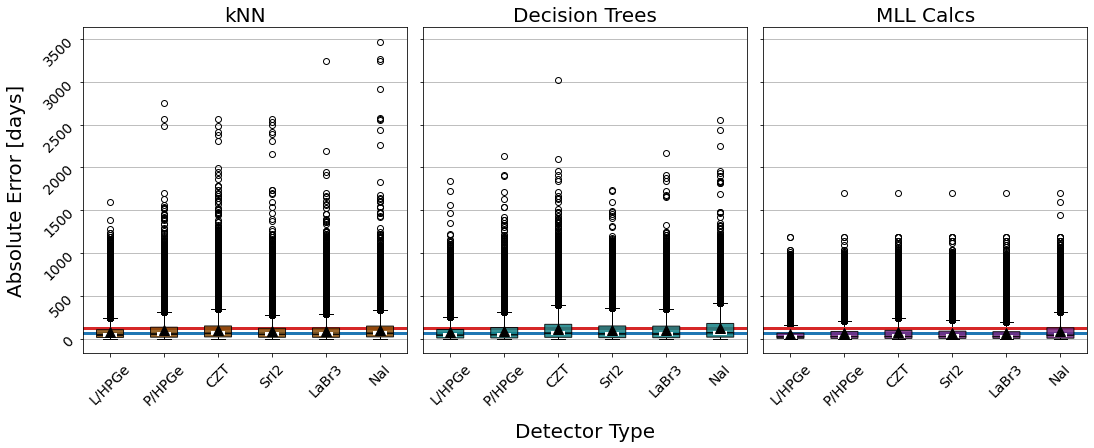
\includegraphics[width=0.92\textwidth]{./chapters/exp2/abserror_boxplots_outliers_short_cool.png}
    \caption{Time since irradiation prediction performance box plots for short energy windows list.}
    \label{fig:coolboxflyB}
  \end{subfigure}
  \vskip\baselineskip
  \begin{subfigure}[b]{\textwidth}
    \centering
    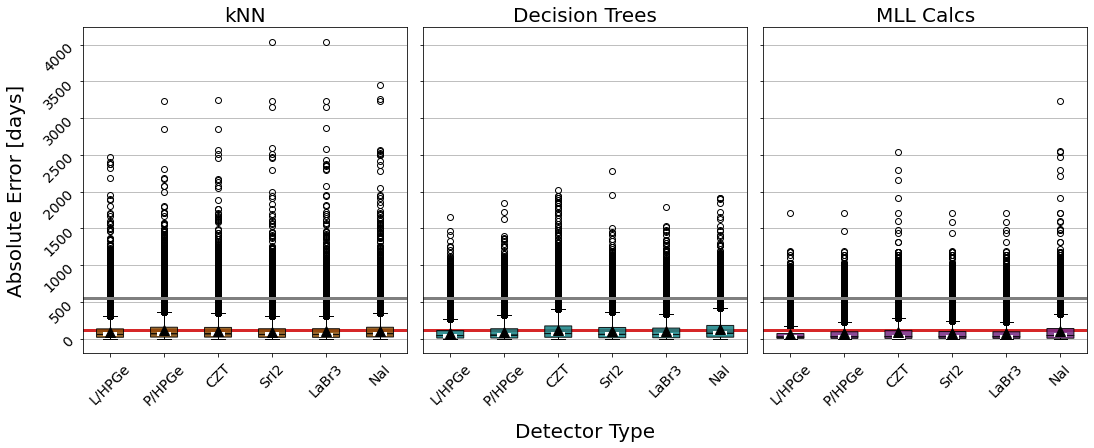
\includegraphics[width=0.92\textwidth]{./chapters/exp2/abserror_boxplots_outliers_long_cool.png}
    \caption{Time since irradiation prediction performance box plots for long energy windows list.}
    \label{fig:coolboxflyC}
  \end{subfigure}
  \caption{Prediction performance of time since irradiation for six detectors as 
           shown by box plots.}
  \label{fig:coolboxfly}
\end{figure}

